\section{Results}
\label{sec:results}

\subsection{Delaunay algorithms}
Firstly, the runtime of the Delaunay algorithms has been measured.
This is done by recursively adding $n$ points to the initial triangulation.

\begin{figure}
    \centering
    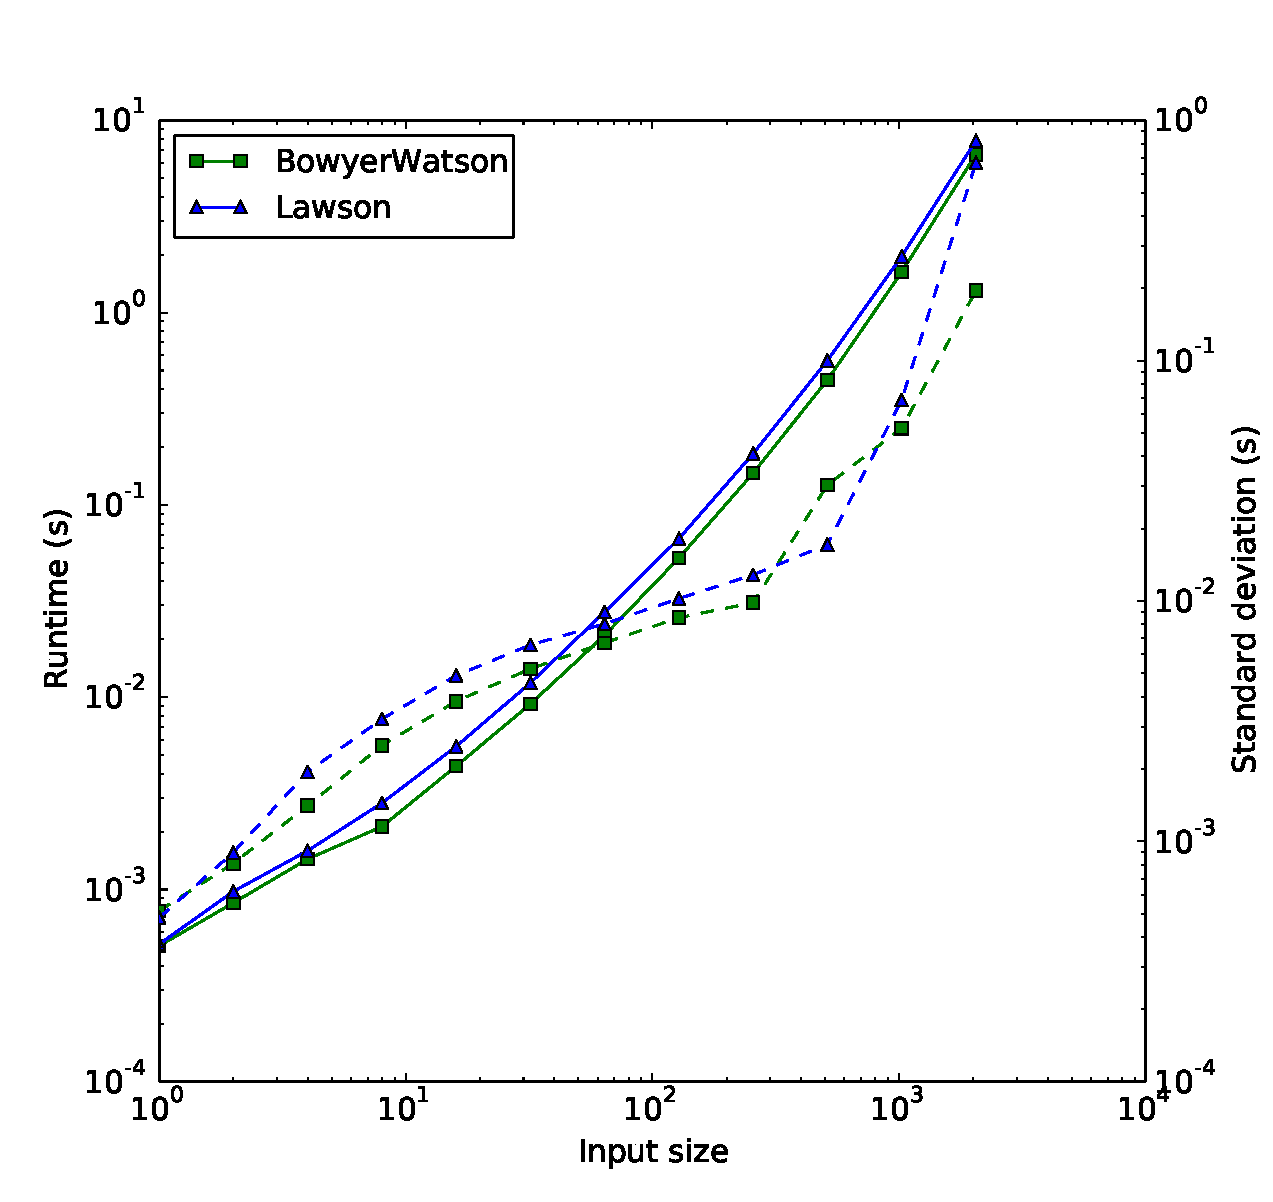
\includegraphics[width=\columnwidth]{../images/runtime.pdf}
    \caption{Runtime comparison of Lawson's and Bowyer-Watson's algorithm.}
    \label{fig:result_runtime}
\end{figure}

\begin{figure}
    \centering
    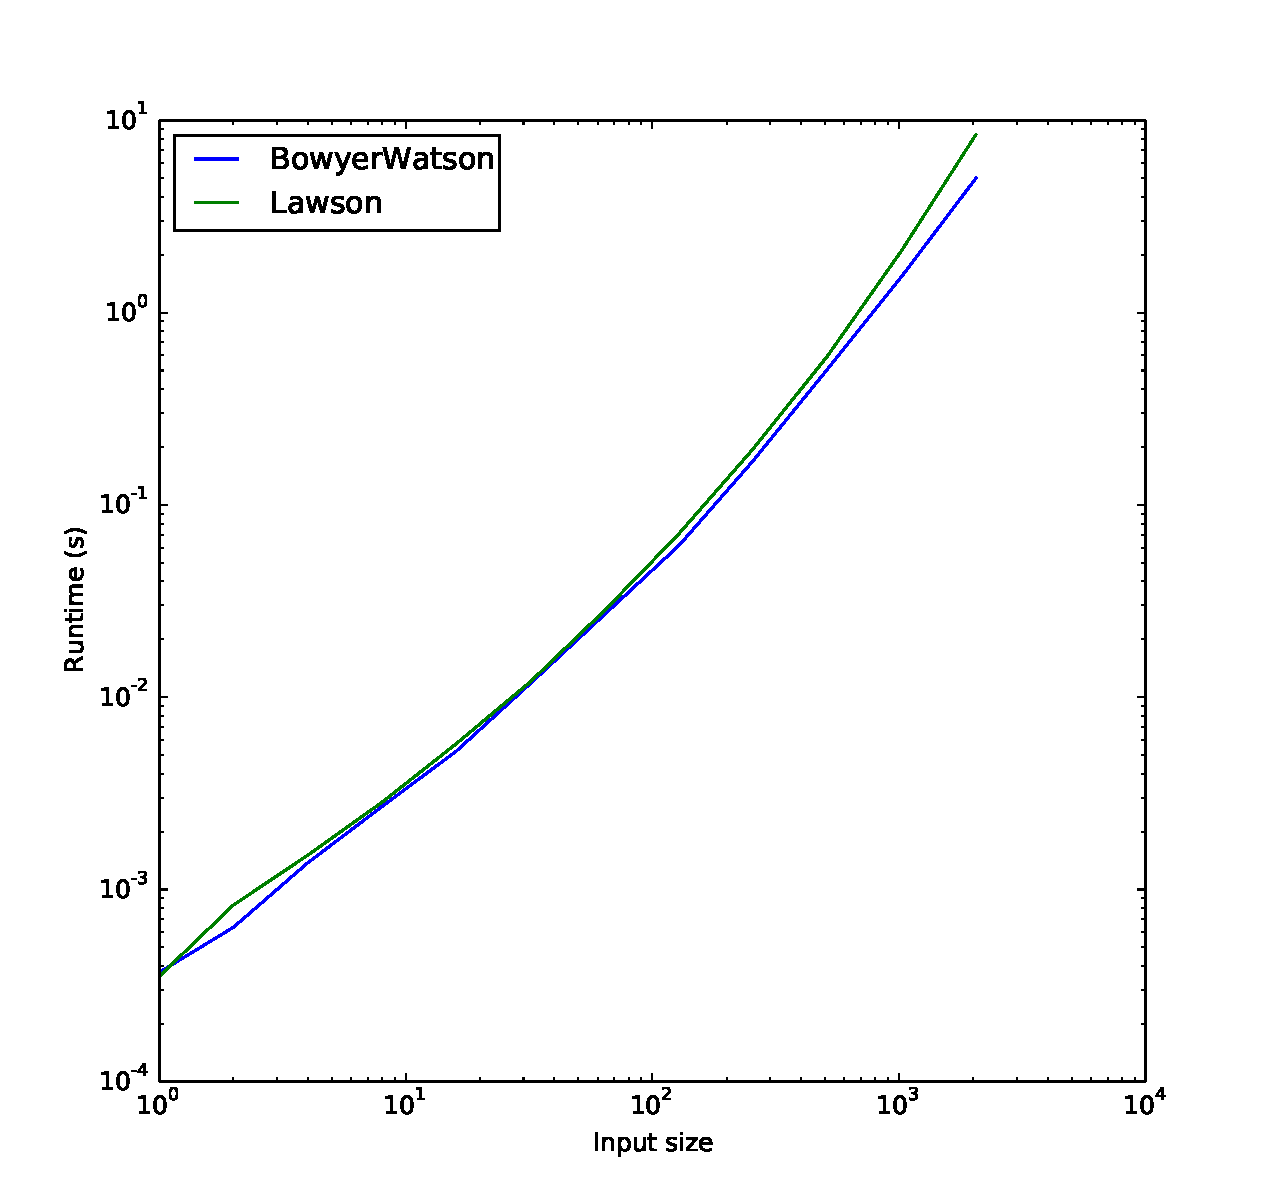
\includegraphics[width=\columnwidth]{../images/runtime_segments.pdf}
    \caption{Like \figref{fig:result_runtime}, but now including 10 randomly placed PSLG boundary segments.}
    \label{fig:result_runtimeSegments}
\end{figure}


\subsection{Ruppert's refinement algorithm}



\begin{figure}
    \centering
    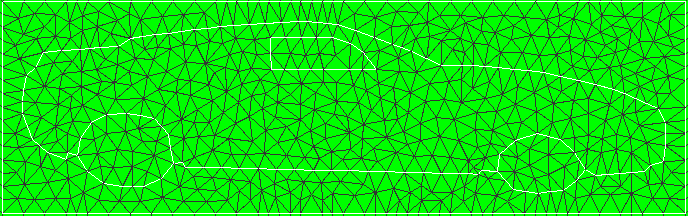
\includegraphics[width=\columnwidth]{../images/Car_Ruppert20.png}
    \caption{Triangulation generated using Ruppert's refinement algorithm for a car. The white lines are PSLG boundary elements.
    The criterea were set to a minimum angle of 20$\degr$ and a maximum area of 200.}
    \label{fig:result_Car20}
\end{figure}

\begin{figure}
    \centering
    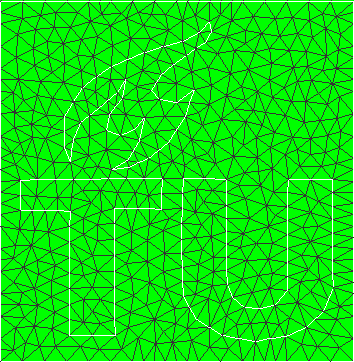
\includegraphics[width=\columnwidth]{../images/TU_Ruppert20.png}
    \caption{Triangulation generated using Ruppert's refinement algorithm for the TU Delft logo. The white lines are PSLG boundary elements.
    The criterea were set to a minimum angle of 20$\degr$ and a maximum area of 200.}
    \label{fig:result_TU20}
\end{figure}